\chapter{Kapcsolódó kutatások}
\label{ch:related_research}

\section{Hulladékdetektálási módszerek}

Számos kutatás készült már a hulladékdetektálás témájában. Az én kutatásom a Térinformatikai kutatólabor munkájára épül \cite{magyar2023}, ahol egy Random Forest modell került betanításra, hulladékdetektálás céljából. A kutatásban PlanetScope és Sentinel-2 műholdfelvételeket használtak. Ez a cikk rakta le az alapjait az én kutatásomnak is, melyben ezeken az eredményeken javítok. A cikkben további lehetséges munkaként említésre kerül a modell több adattal való tanítása, illetve a képfeldolgozás gyorsítása. A dolgozatom mindkét feladattal foglalkozik,  A dolgozatomban csak a PlanetScope felvételek kerülnek felhasználásra, mivel a magasabb felbontású felvételek könnyebben lehetővé teszik a tanítóadatok előállítását, hiszen jobban lehet látni a hulladéklerakókat rajtuk.

\cite{sakti2023}-ben Sentinel-2 műholdfelvételeken tanítottak be egy Random Forest modell-t azzal a céllal, hogy egy indonéziai folyóban detektáljanak hulladékot. A cikkben bevezetik az "Adjusted Plastic Index"-et, mellyel a vegetáció, föld és épületek közötti zajt csökkentik. Ennek az indexnek a kiszámításához a Sentinel-2 műhold piros, közeli infravörös (NIR), illetve rövid hullámhosszú közeli infravörös (SWIR) sávokat használták fel. Validációnak Pleiades műholdképeket és drónfelvételeket klasszifikáltak Mahalanobis távolság gépi tanulási módszerrel (\ref{fig:sakti} ábra) . A módszer növényzeten és vízen rendre 88\%, illetve 85\% pontosságot ért el és épületeken, törmeléken és földön rendre 62\%, 53\%, illetve 21\% pontossággal tudta a hulladékot detektálni. A cikk szerint az utóbbi három adattípuson azért visszafogottabbak az arányok, mert a spektrális értékei az épületeknek, a földnek és a törmeléknek nagyon hasonlítanak.

\begin{figure}[H]
	\centering
	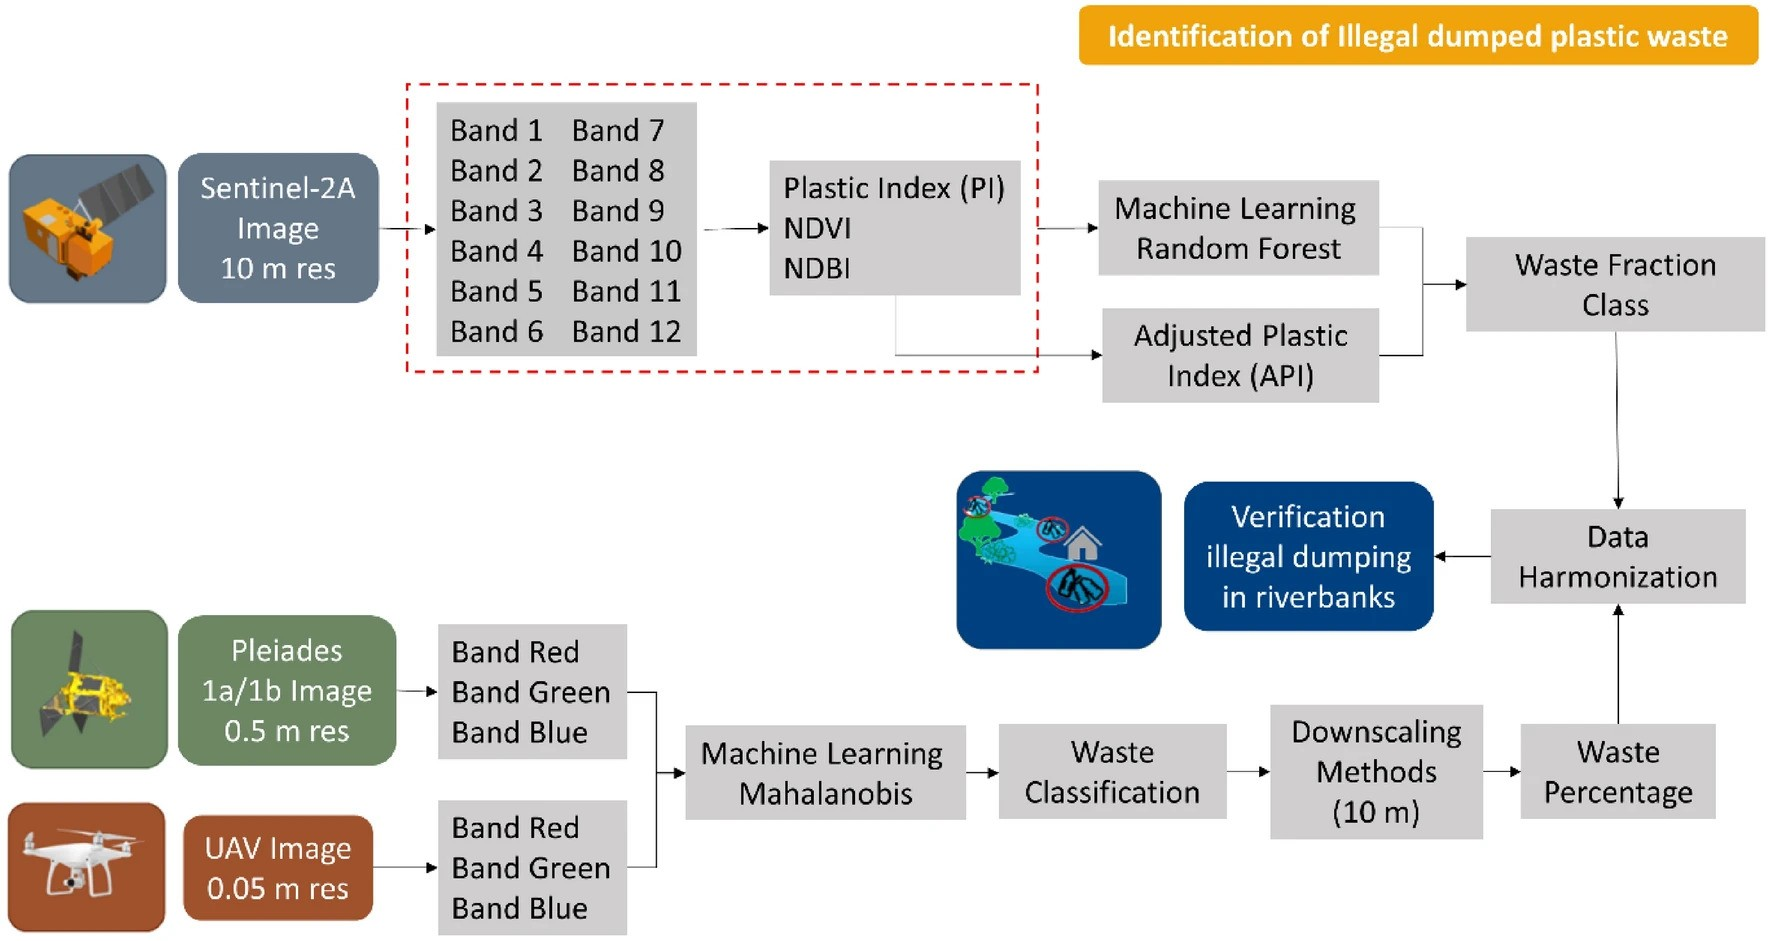
\includegraphics[width=0.6\textwidth,frame]{sakti}
	\caption{Hulladékdetektálás "Adjusted Plastic Index", Random Forest és Mahalanobis távolság segítségével \cite{sakti2023}}
    \label{fig:sakti}
\end{figure}


\cite{goncalves2022}-ben Spectral Angle Mapping módszert alkalmaztak multispektrális drónfelvételeken, egy Portugál tengerparton. A célja a kutatásnak az volt, hogy a tengerparton kimosott hulladékot detektálják és klasszifikálják. A módszer alkalmazásához referencia értékeket állítottak elő azzal, hogy elhelyeztek különböző anyagokból álló hulladékot a homokba, és ezekről drónfelvételt készítettek (\ref{fig:goncalves} ábra). Ezzel a módszerrel képesek voltak detektálni és klasszifikálni nem csak homok fölött található hulladékot, hanem a homokban félig elásott hulladékot is. A 472 kézzel előállított tesztadatból volt a 268 True Positive(57\% összesen), 96 volt a False Positive és 204 volt a False Negative.

\begin{figure}[H]
	\centering
	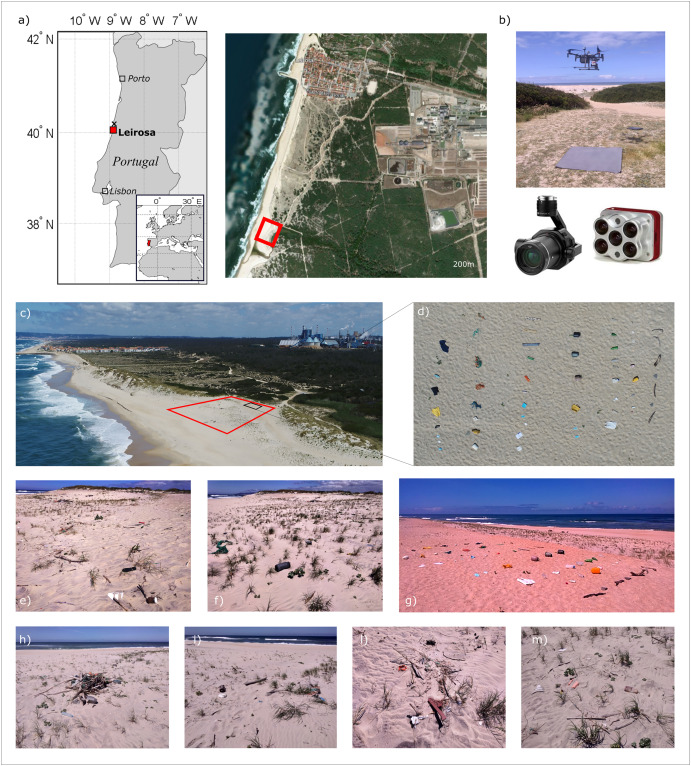
\includegraphics[width=0.6\textwidth,frame]{goncalves}
	\caption{Spectral angle mapping referencia adatainak előállítása \cite{goncalves2022}}
    \label{fig:goncalves}
\end{figure}

\cite{lanorte2017}-ben mezőgazdasági hulladékdetektálásra használtak egy Support Vector Machine modellt, Landsat 8 műholdfelvételeken. A szenzor Kék, Zöld, Piros, NIR, SWIR 1, SWIR 2 és CIRRUS sávját használták a tanítóadatok és tesztadatok előállítására. Ezután véletlenszerűen szétválasztották az adatokat tanítóadatokra és tesztadatokra. A következő osztályokra bontották az adatokat: Hálók, műanyag takarók, föld, növényzet, gyümölcsöskert, olajfás kert, város, fa, fás föld. A modell a tesztadatokat összességében 94\%-os pontossággal tudta klasszifikálni, ahol a legrosszabb arányokat az olajfás kert érte el 77.78\%-os pontossággal.

\cite{zeng2019}-ben a hiperspektrális adatokon tanítottak be egy felügyelt és egy felügyeletlen gépi tanulási módszert. A működési elv az, hogy a felügyelt módszerrel klasszifikálják a hulladékkal szennyezett területeket, míg a felügyeletlen módszerrel megbecsülik a hulladékkal szennyezett terület kerületét(\ref{fig:zeng} ábra). Ők 99.89\%-os kappa együtthatóval tudtak hulladékot detektálni \todo{Átnézni mégegyszer a cikket és átvizsgálni az adatok helyességét}.

\begin{figure}[H]
	\centering
	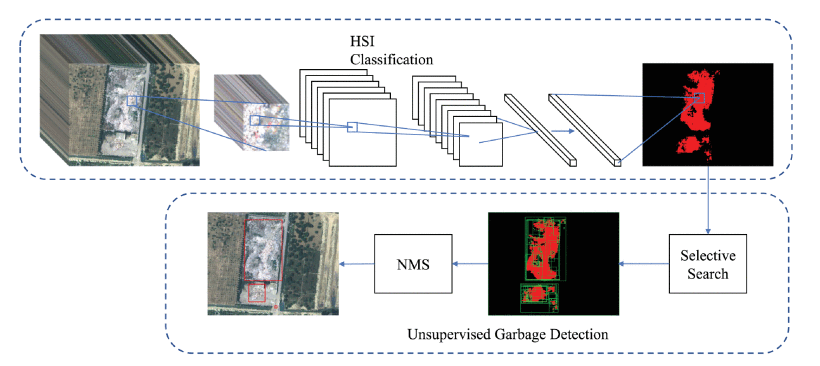
\includegraphics[width=0.6\textwidth,frame]{zeng}
	\caption{Az MSCNN működési elve \cite{zeng2019}}
    \label{fig:zeng}
\end{figure}

\section{Random Forest}

A Random Forest egy felügyelt gépi tanulási módszer, mely magas pontossággal tud rátanulni a tanítóadatokra (túltanulás nélkül), és jól kezeli a zajt \cite{breiman2001}. A módszer több, különbözően paraméterezett döntési fa felépítéséből kapta a nevét: miután felépítettük ezt a "döntési fa erdőt", az adatokat úgy lehet osztályozni, hogy egy többségi szavazást hajtunk végre az összes fa eredménye szerint (\ref{fig:random-forest} ábra). A fák felépítéséhez több stratégia létezik, és ezen stratégiák alapján lehet finomhangolni a modell pontosságát és méretét. Az utóbbit fontos szem előtt tartani, tekintve arra, hogy elég sok adat esetén a modell mérete lényegesen megnőhet helyes paraméterezés hiányában. Az ilyen paraméterek például a fák maximum mélysége, a fáknak átadott részadathalmaz dimenziói, egy csúcs kettéválasztásának a kritériumjai, a tanítóadatok súlyai stb. A kutatásomban ezt a modellt tanítom be, illetve paraméterezem azzal a céllal, hogy megbízható klasszifikációt tudjon biztosítani. A modell minden képkockát osztályozni fog, így a bemeneti adatok az adott terület spektrális sávjai, illetve indexei. 

